\documentclass[tikz,border=8pt]{standalone}
\usepackage[utf8]{inputenc}
\usepackage[OT4,plmath]{polski}
\usepackage{amsmath}
\usetikzlibrary{patterns}
\begin{document}
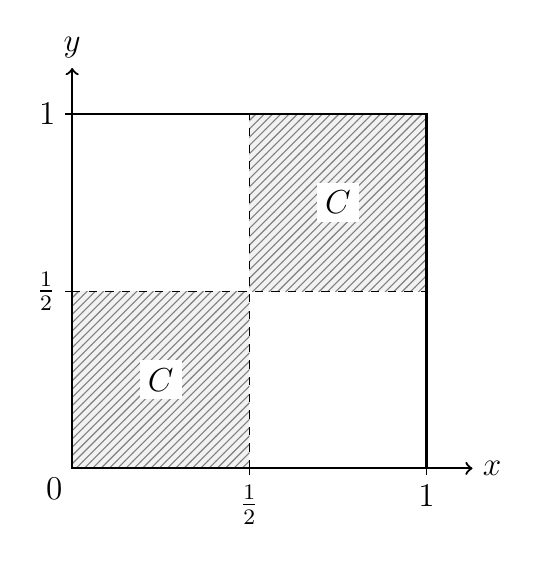
\begin{tikzpicture}[x=4.5cm,y=4.5cm,font=\large]
  \fill[black!5] (0,0) rectangle (.5,.5);
  \fill[black!5] (.5,.5) rectangle (1,1);
  \fill[pattern=north east lines,pattern color=black!50]
    (0,0) rectangle (.5,.5);
  \fill[pattern=north east lines,pattern color=black!50]
    (.5,.5) rectangle (1,1);
  \draw[thick] (0,0) rectangle (1,1);
  \draw[dashed] (.5,0)--(.5,1) (0,.5)--(1,.5);
  \draw[->,thick] (0,0)--(1.13,0) node[right] {$x$};
  \draw[->,thick] (0,0)--(0,1.13) node[above] {$y$};
  \node[below left] at (0,0) {$0$};
  \foreach \v/\lab in {.5/{\frac12},1/{1}} {
    \draw (\v,0)--(\v,-.02) node[below] {$\lab$};
    \draw (0,\v)--(-.02,\v) node[left] {$\lab$};
  }
  \node[fill=white,inner sep=3pt] at (.25,.25) {$C$};
  \node[fill=white,inner sep=3pt] at (.75,.75) {$C$};
\end{tikzpicture}
\end{document}
